\documentclass[tikz,border=5mm]{standalone}
\tikzset{pics/hackenbush/.style args={#1|#2}{
code={
\begin{scope}[local bounding box=#1]
\draw[line width=2pt] (0,0)--++(90:#2) node[left]{};
\end{scope}
}}}
\begin{document}
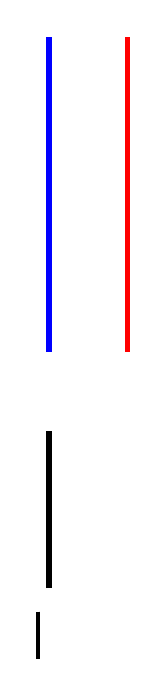
\begin{tikzpicture}
\pic[blue] {hackenbush={A|4}};
\pic[right=1cm,red] {hackenbush={B|4}};
\pic[below=3cm] {hackenbush={C|2}};
\draw[ultra thick,black] ([yshift=-.3cm]C.south) --++(-90:.6);
\draw[ultra thick,black] ([yshift=-.3cm]C.south) --++(-90:.6);
\end{tikzpicture}
\end{document}